\subsubsection{Adapted SAGAT}
\label{subsubsec:results_adapted_sagat_2}

Table \ref{tab:sagat_table_noBase} presents the SAGAT score of all participants. The corresponding barplot is presented in Figure \ref{fig:barplot_sagat_avg_4_scene_blind_sight}.


\begin{table}[!htb]
\centering
\caption{SAGAT global score felled by the participants.}
\label{tab:sagat_table_noBase}
\begin{tabular}{lllrrrrr}
\toprule
    &       &        &  Audio & \begin{tabular}[c]{@{}l@{}}Haptic\\ Belt\end{tabular} & \begin{tabular}[c]{@{}l@{}}Virtual\\ Cane\end{tabular} & Mixture \\
Participant & \begin{tabular}[c]{@{}l@{}}Visual\\ Condition\end{tabular} & Round &        &                                                       &                                                        &         \\
\midrule
001C & Blind & First &  5.500 &                                                 5.330 &                                                  5.830 &   3.500 \\
    &       & Return &  6.500 &                                                 8.500 &                                                  5.500 &   5.500 \\
002C & Blind & First &  4.500 &                                                 3.990 &                                                  4.500 &   6.250 \\
    &       & Return &  5.000 &                                                 4.000 &                                                  6.500 &   8.500 \\
003C & Blind & First &  7.500 &                                                 7.490 &                                                  4.660 &   9.000 \\
    &       & Return & 10.000 &                                                 8.500 &                                                  9.000 &   9.000 \\
004C & Blind & First &  6.000 &                                                 7.660 &                                                  4.990 &   6.500 \\
    &       & Return &  6.000 &                                                 9.250 &                                                  7.250 &   9.000 \\
001 & Sight & First &  4.500 &                                                 4.330 &                                                  2.660 &   6.500 \\
    &       & Return &  6.000 &                                                 5.000 &                                                  5.000 &   4.500 \\
003 & Sight & First &  6.750 &                                                 5.990 &                                                  3.990 &   6.750 \\
    &       & Return &  6.000 &                                                 7.250 &                                                  6.250 &   7.500 \\
004 & Sight & First &  7.250 &                                                 7.990 &                                                  5.990 &   8.250 \\
    &       & Return &  7.750 &                                                 9.500 &                                                  8.250 &   7.000 \\
005 & Sight & First &  3.000 &                                                 3.160 &                                                  3.990 &   4.000 \\
    &       & Return &  3.750 &                                                 3.000 &                                                  2.000 &   6.000 \\
\bottomrule
\end{tabular}
\end{table}



Figure \ref{fig:barplot_sagat_avg_4_scene_blind_sight}. shows that the SAGAT score for sighted participants is on average lower than that of blind participants, which is expected as they are not used to navigate without vision. Also, the increase in situation awareness from the first to the return round is lower. In the case of the mixture method, the SAGAT score did not improve at all. For both groups, the ‘virtual cane’ was the method with lowest score in the first round.

\begin{figure}[!htb]
    \centering
    \begin{minipage}{\textwidth}
        \centering
        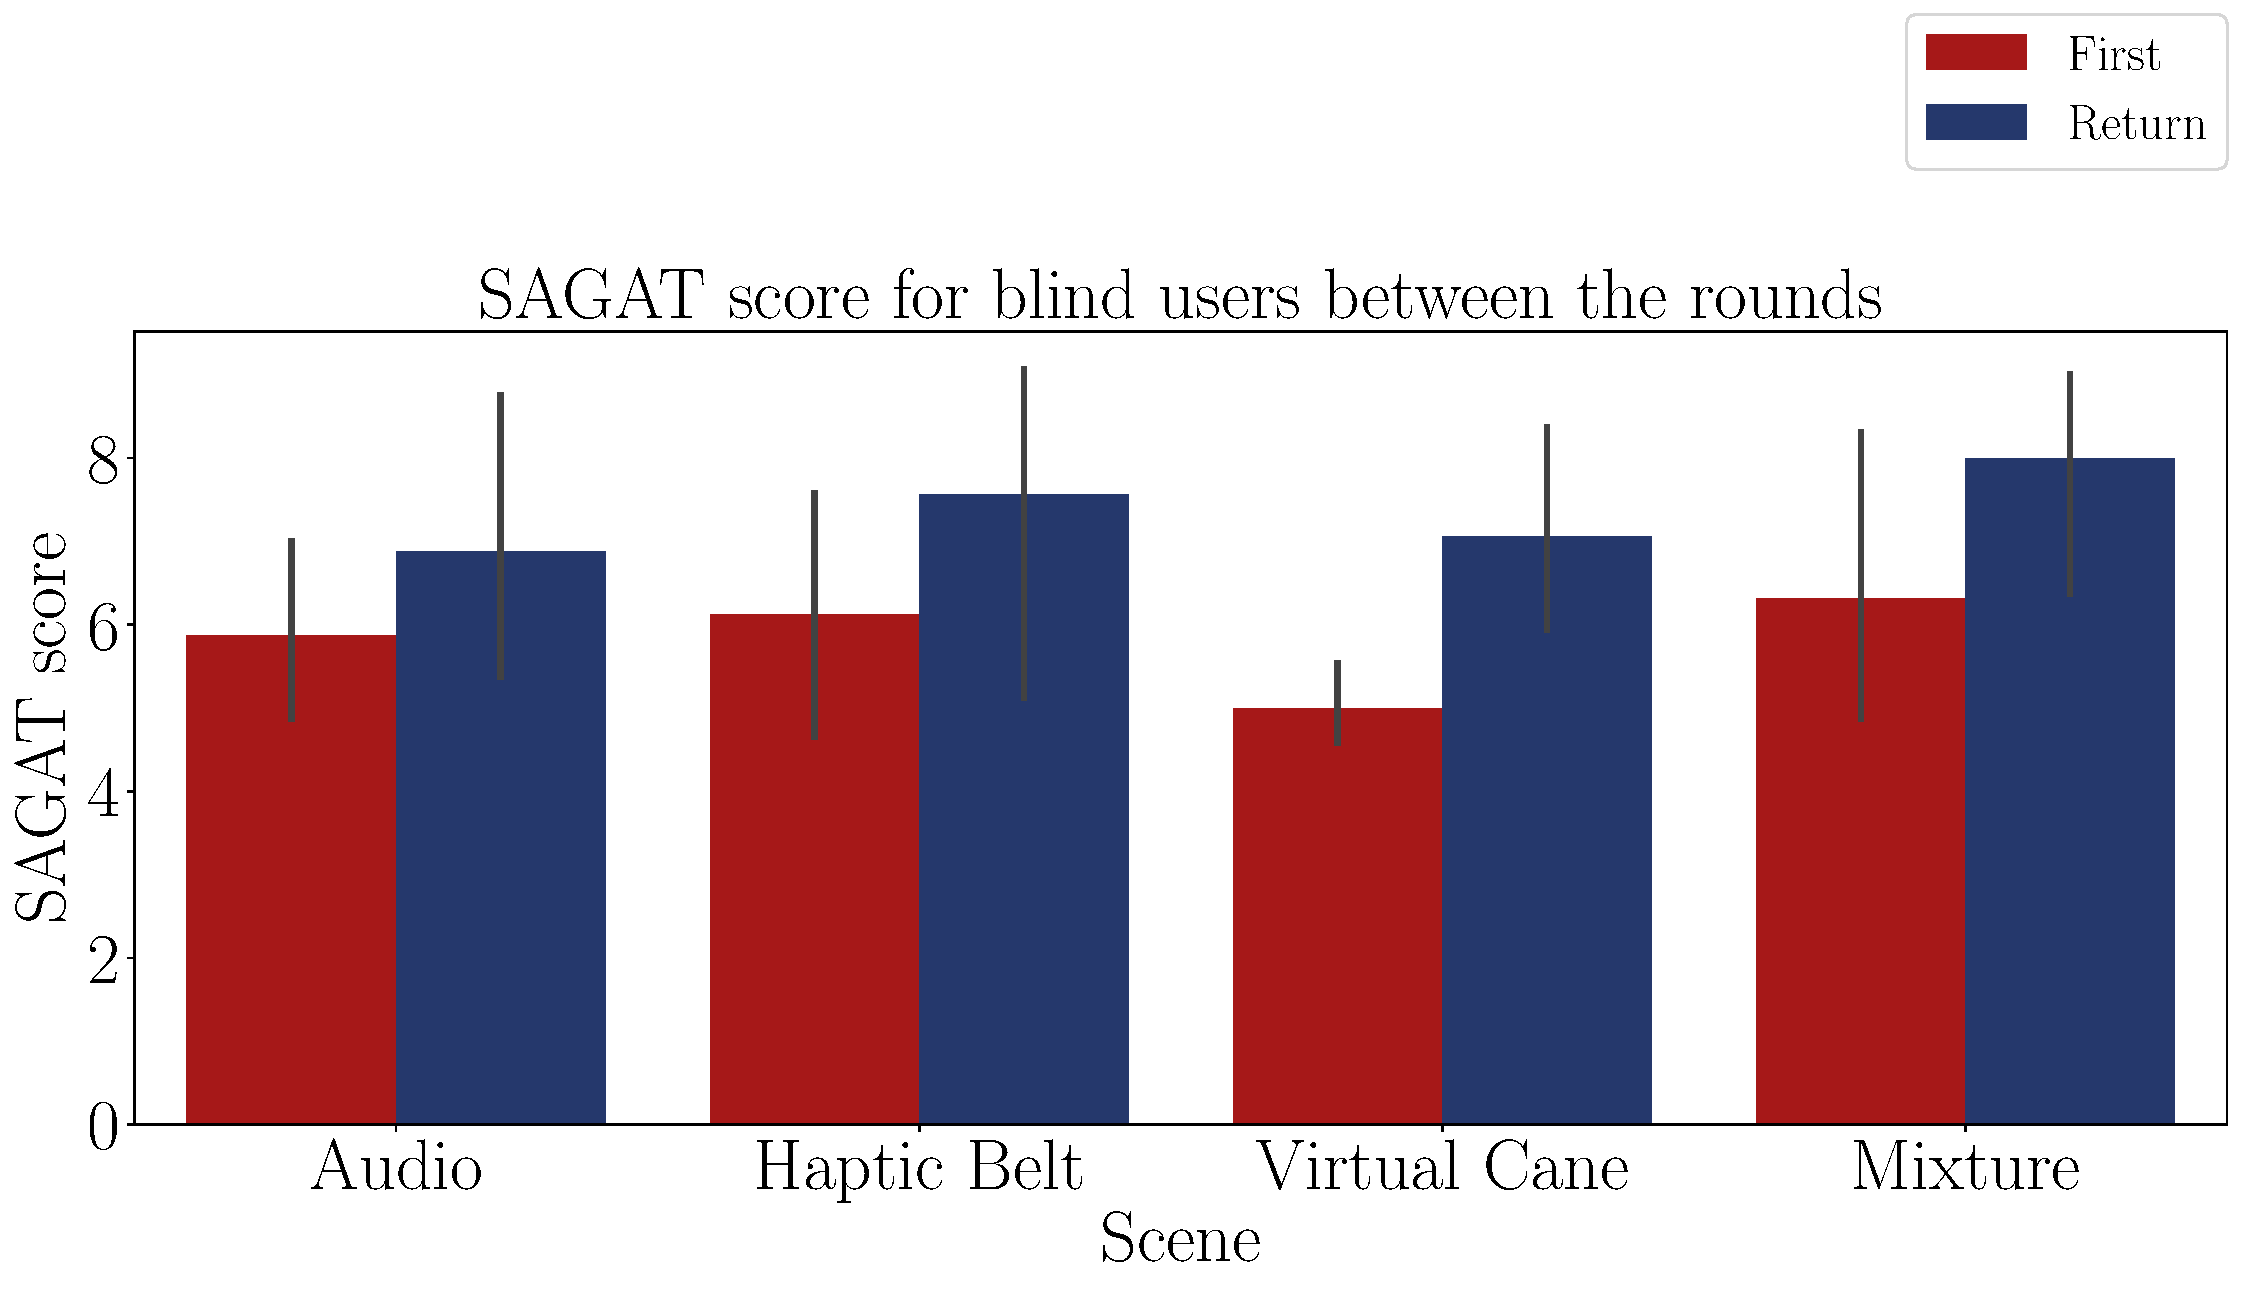
\includegraphics[width = \textwidth]{Resultados/Sagat/Figuras/pdf/barplot_sagat_avg_4_scene_blind.pdf}
        \subcaption{Blind participants.}
        \label{fig:barplot_sagat_avg_4_scene_blind}
    \end{minipage}
    \begin{minipage}{\textwidth}
        \centering
        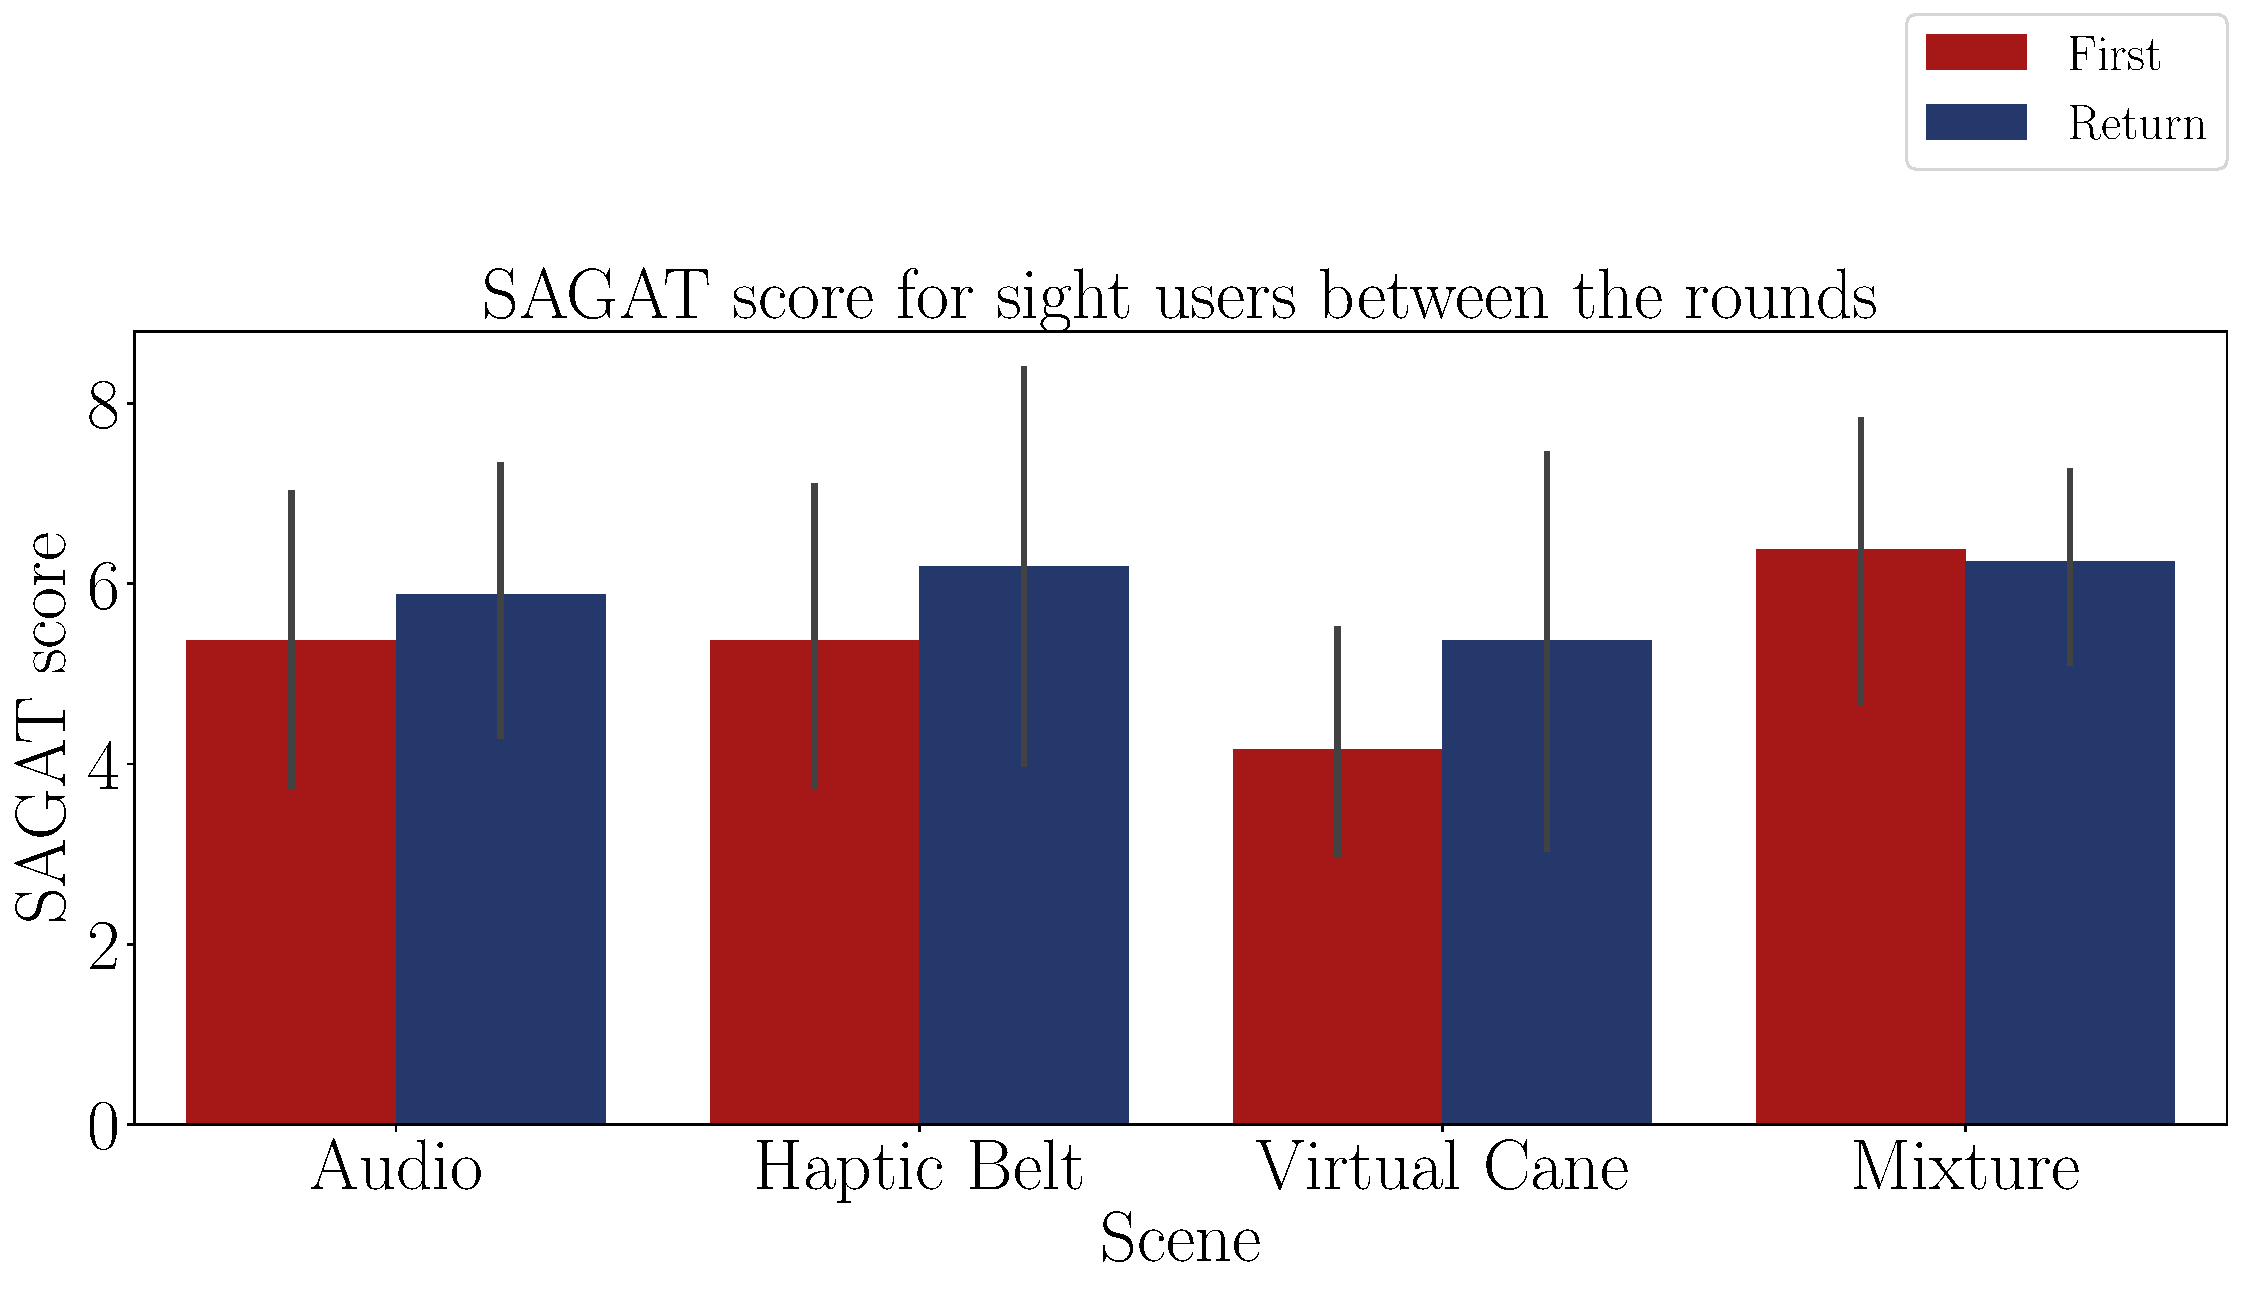
\includegraphics[width = \textwidth]{Resultados/Sagat/Figuras/pdf/barplot_sagat_avg_4_scene_sight.pdf}
        \subcaption{Sight participants.}
        \label{fig:barplot_sagat_avg_4_scene_sight}
    \end{minipage}
    \caption{Barplot of the SAGAT score on each method and round.}
    \label{fig:barplot_sagat_avg_4_scene_blind_sight}
\end{figure}

Figures \ref{fig:boxplot_sagat_4_scene} and \ref{fig:boxplot_sagat_4_rounds} bring the boxplots. According to Figure \ref{fig:boxplot_sagat_4_scene}, both groups presented a higher situation awareness with ‘mixture’ and ‘haptic’. On the other hand, Figure \ref{fig:boxplot_sagat_4_rounds} confirms that the difference between the rounds is greater for blind participants. 

\begin{figure}[!htb]
    \centering
    \begin{minipage}{0.45\textwidth}
        \centering
        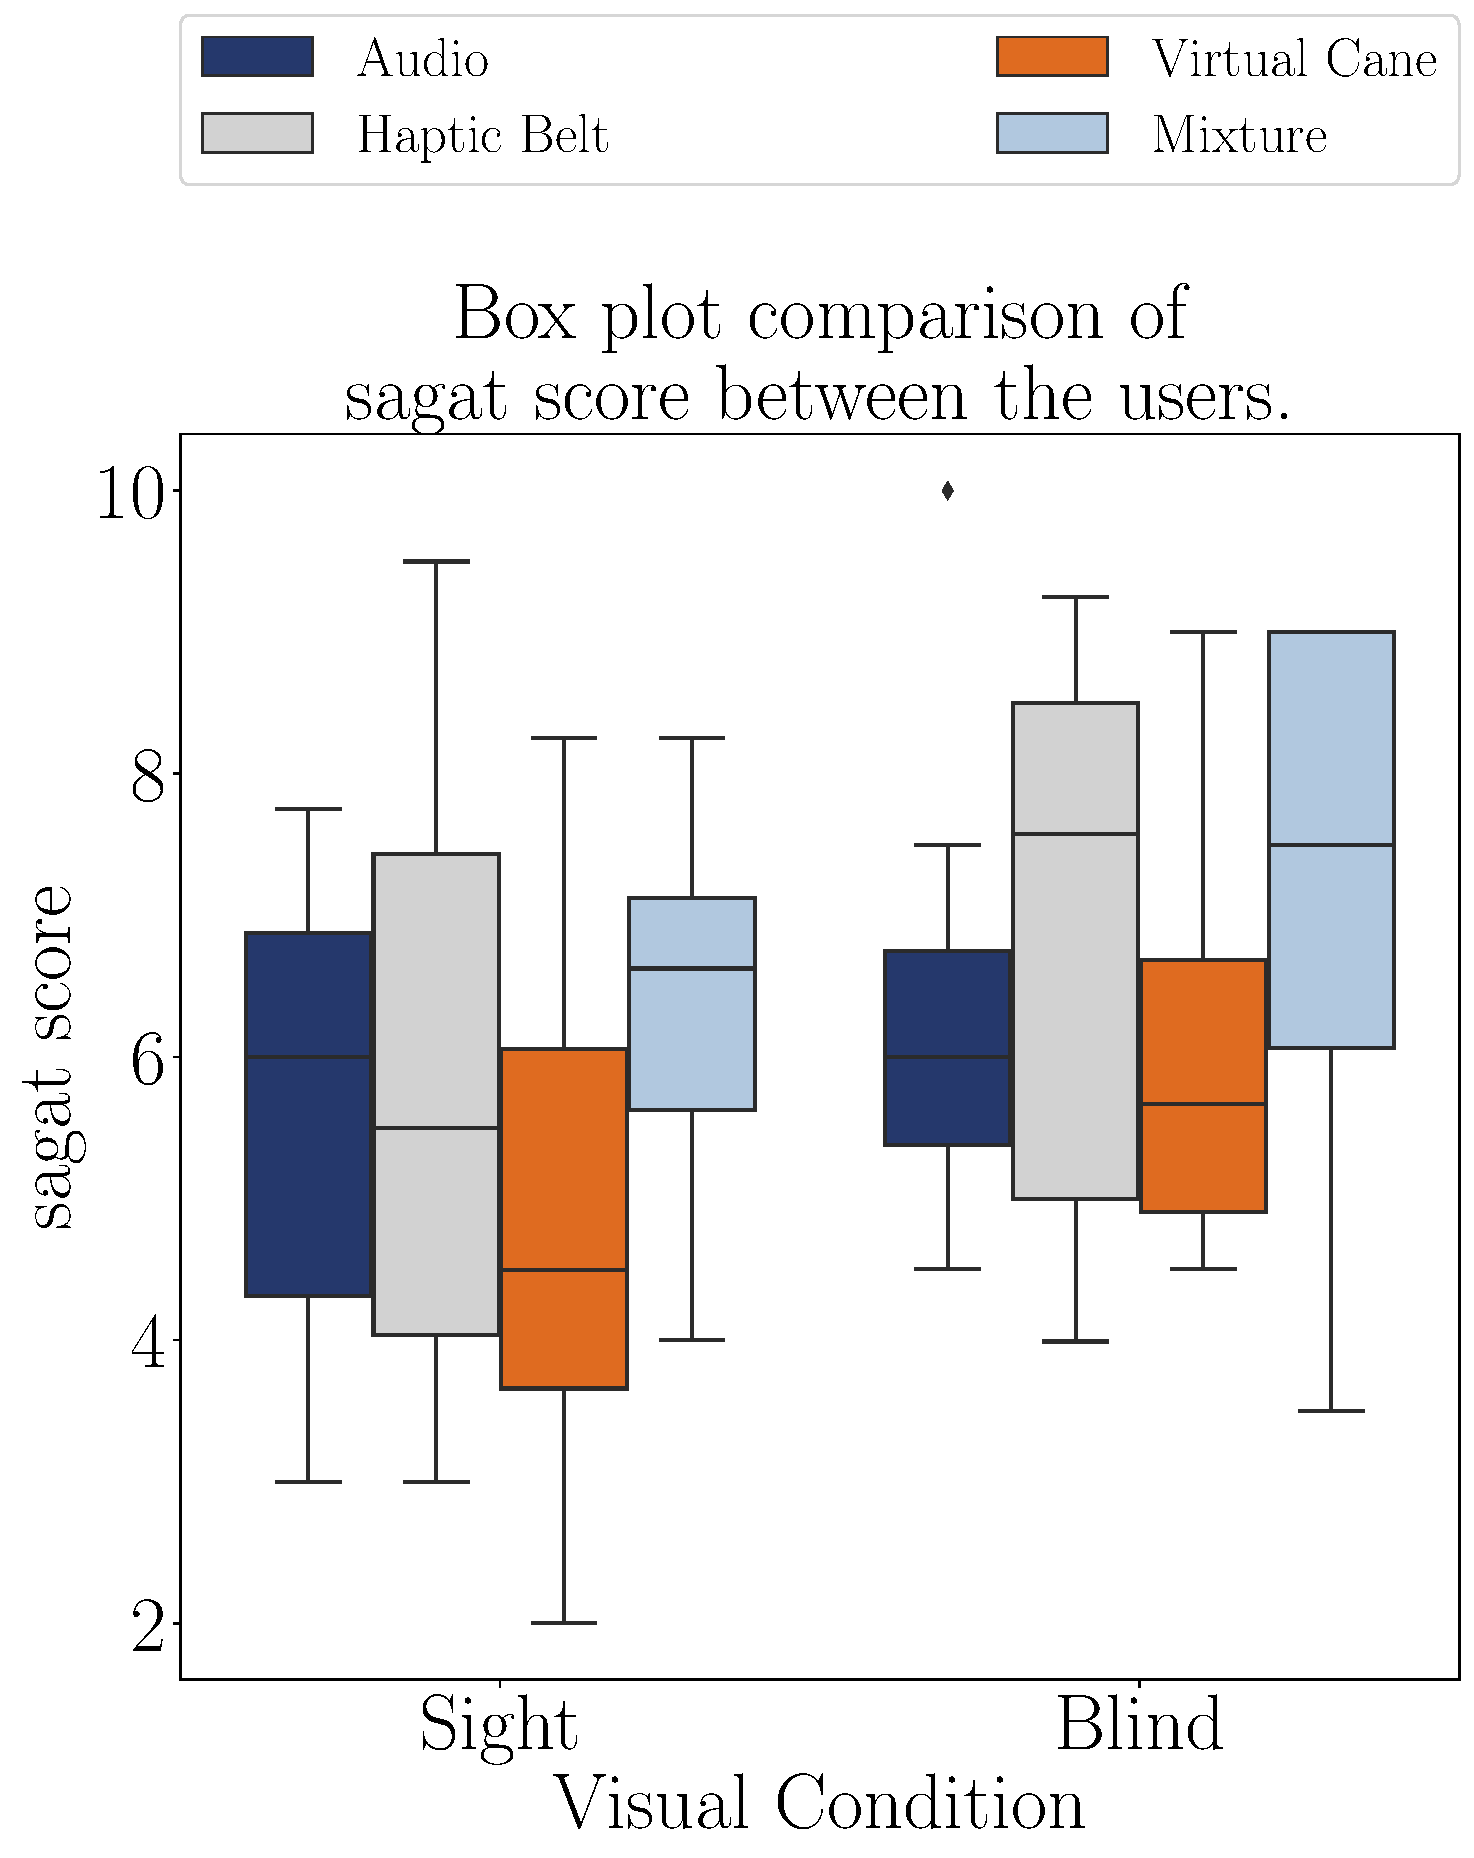
\includegraphics[width = \textwidth]{Resultados/Sagat/Figuras/pdf/boxplot_sagat_4_scene.pdf}
        \caption{Boxplot of the Sagat score of the participants grouped by method.}
        \label{fig:boxplot_sagat_4_scene}
    \end{minipage}
    \begin{minipage}{0.075\textwidth}
        \hfill
    \end{minipage}
    \begin{minipage}{0.45\textwidth}
        \centering
        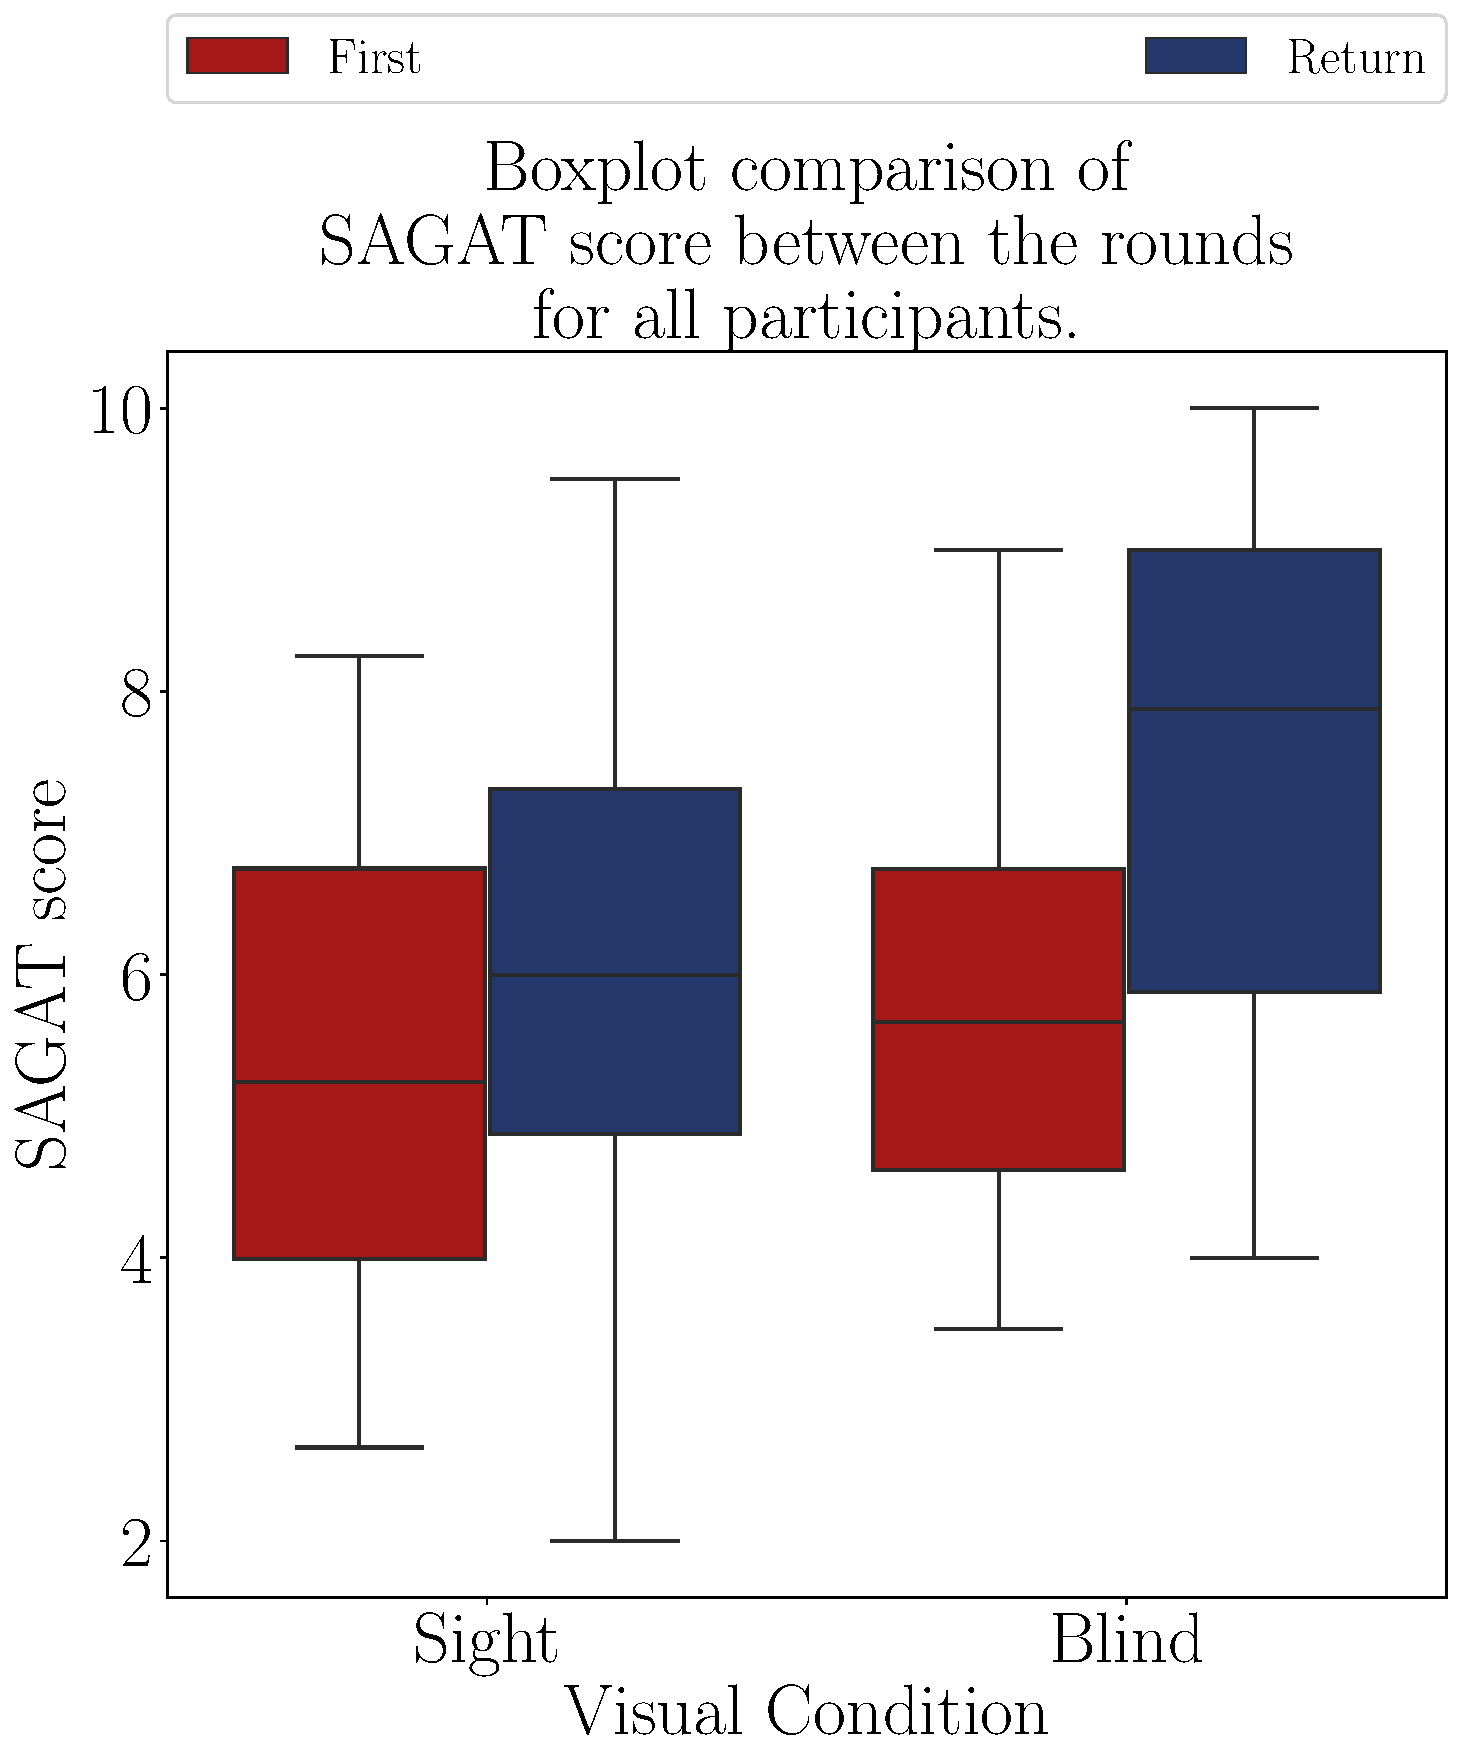
\includegraphics[width = \linewidth]{Resultados/Sagat/Figuras/pdf/boxplot_sagat_4_rounds.pdf}
        \caption{Boxplot of the Sagat score of the participants grouped by round.}
        \label{fig:boxplot_sagat_4_rounds}
    \end{minipage}
\end{figure}

Figures \ref{fig:qqplot_sagat_avg_two_way_sight} and \ref{fig:residplot_sagat_avg_two_way_sight} brings the QQ plot and residual distribution. It is clear that the residuals variance is not equal among the participants. Table \ref{tab:blocanova_sagat_avg_two_way_blind_sight} brings the p-value from ANOVA. While for blind participants the round is a significant factor and the method is not, for sighted participants the result is the opposite, showing a significant influence of the method and not of the round.

\begin{table}[!htb]
    \caption{Anova p-value for the SAGAT score on each method}
    \label{tab:blocanova_sagat_avg_two_way_blind_sight}
\begin{minipage}{0.45\textwidth}
    \subcaption{Blind participants}
    
\centering
\begin{tabular}{ll}
\toprule
          Source & P-Value \\
\midrule
    \    Methods &   0.277 \\
     \    Rounds & 0.002** \\
\    Interaction &   0.834 \\
\bottomrule
\end{tabular}

\end{minipage}
\begin{minipage}{0.45\textwidth}
    \subcaption{Sight participants}
    
\centering
\begin{tabular}{ll}
\toprule
          Source & P-Value \\
\midrule
    \    Methods & 0.035** \\
     \    Rounds &   0.095 \\
\    Interaction &   0.578 \\
\bottomrule
\end{tabular}
    
\end{minipage}
\end{table}


\begin{figure}[!htb]
    \centering
    %\vspace{-15.0cm}
    \begin{minipage}{0.45\textwidth}
        \centering
        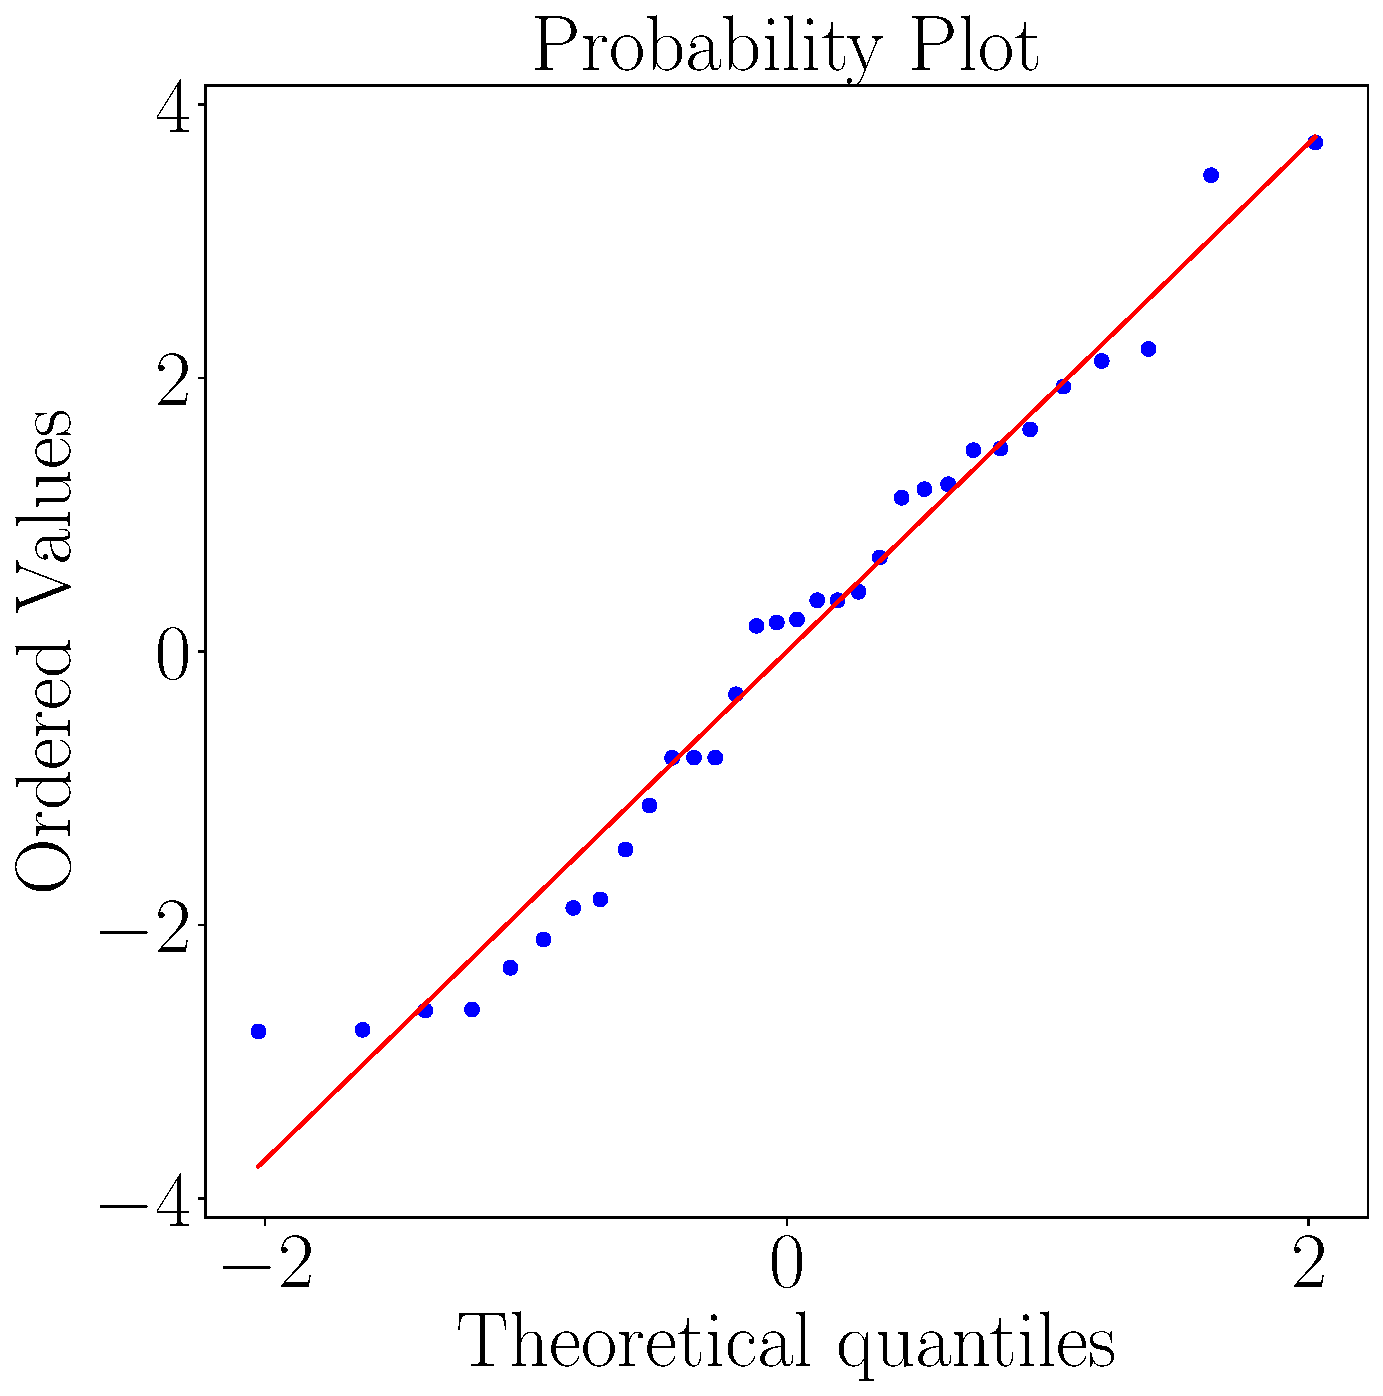
\includegraphics[width = \textwidth]{Resultados/Sagat/Figuras/pdf/qqplot_sagat_avg_two_way_sight.pdf}
        \caption{QQ plot of the mental demand of the sight participants on each method.}
        \label{fig:qqplot_sagat_avg_two_way_sight}
    \end{minipage}
    \begin{minipage}{0.075\textwidth}
        \hfill
    \end{minipage}
    \begin{minipage}{0.45\textwidth}
        \centering
        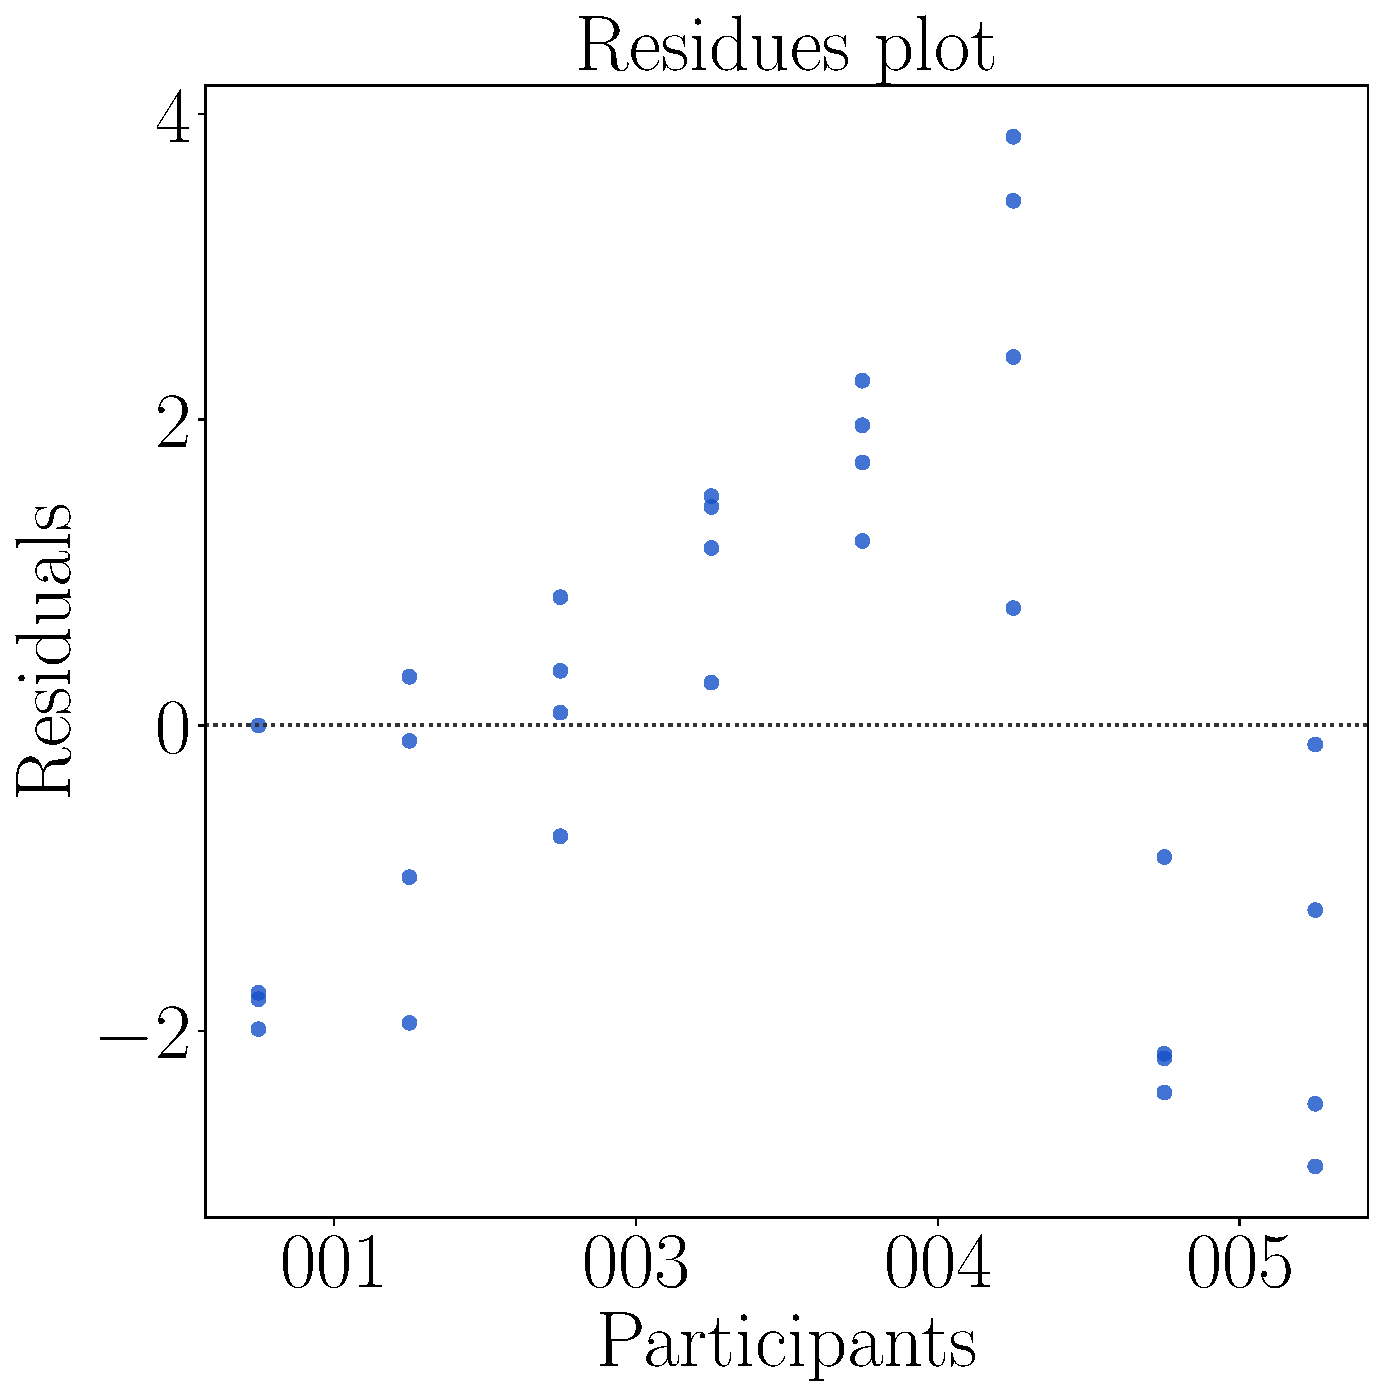
\includegraphics[width = \textwidth]{Resultados/Sagat/Figuras/pdf/residplot_sagat_avg_two_way_sight.pdf}
        \caption{Residual plot of the mental demand score the sight participants on each method.}
        \label{fig:residplot_sagat_avg_two_way_sight}
    \end{minipage}
\end{figure}

%%%%%%%%%%%%%%%%%%%%%%%%%%%%%%%%%%%%%%%%%%%%%%%%%%%%%

\FloatBarrier